%!TEX root = <uw-ethesis.tex>
% T I T L E   P A G E
% -------------------
% Last updated May 24, 2011, by Stephen Carr, IST-Client Services
% The title page is counted as page `i' but we need to suppress the
% page number.  We also don't want any headers or footers.
\pagestyle{empty}
\pagenumbering{roman}

% The contents of the title page are specified in the "titlepage"
% environment.
\begin{titlepage}
        \begin{center}
        % \vspace*{1.0cm}

        \Large
        {\bf \sc \underline{University Of Waterloo}}
        
        \normalsize
        {\bf \sc Faculty Of Engineering \\
        Mechanical And Mechatronics Engineering} \\

        \vspace*{1.0cm}
        \Large
        {\bf \uppercase{Video Transcoding Rate Prediction using machine learning}}
        
        \vspace*{1.5cm}
        \normalsize
        \begin{figure}[h!]
        \centering
        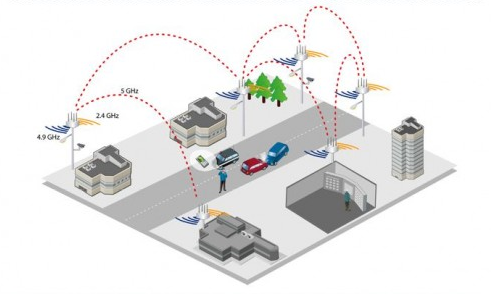
\includegraphics[width=\textwidth]{title}
        \label{fig:tit}
        \end{figure}
        
        \vfill
        {\sc Self Study Report}

        \vspace*{1cm}
        Prepared by\\
        {\sc Satya Prahlada Sthita Prajna Kandarpa \\
        UW ID 20402024 $\vert$ Userid \textit{spspkand} \\ 
        4B Mechatronics Engineering \\
        4 April 2016}

        \end{center}
\end{titlepage}



\cleardoublepage % Ends the current page and causes all figures and tables that have so far appeared in the input to be printed.
% In a two-sided printing style, it also makes the next page a right-hand (odd-numbered) page, producing a blank page if necessary.

% Letter of Submittal%
\begin{flushleft}
    41 Pineslope Crescent\\
    Scarborough, Ontario, Canada\\
    M1E 4M5
    \textit{4 April 2016}
    
    Professor William Melek, Director of Mechatronics Engineering\\
    Department of Mechanical and Mechatronics Engineering\\
    University of Waterloo, Waterloo, Ontario\\
    N2L 3G1
    
    Dear Sir,

    This report, titled "Video Transcoding Rate Prediction using machine learning techniques", was prepared as my 4B Work Report for the University of Waterloo. This report is in fulfillment of the course WKRPT 400.

    I got exposed to some innovative and novel media processing techniques at a startup I worked at which helped pique my interest in audio visual media processing. The purpose of this report is to offer a software based predictive model that can decrease the time required to choose video standards for best transcoding performance without actually performing the transcoding operation between an input and output video standard. Such predictive models are useful for extremely large video transcoding operations, usually done by high profile video streaming and storage sites, where its not feasible to test every possible input/output video standard to pick the best one for a specific platform or operation.
    
    The technical analysis conducted by me for this purpose incorporates machine learning techniques to evaluate the standard video encoding technologies to produce models which are able to predict transcoding rates for some of the most common video codec configurations. In conclusion, this report offers a freely available software based predictive model
    
    This report was written entirely by me and has not received any previous academic credit at this or any other institution. 

    Sincerely,\\
    Satya Prahlada Sthita Prajna Kandarpa\\
    ID 20402024\\
\end{flushleft}
\cleardoublepage

